\documentclass[12pt, letterpaper]{article}

\usepackage[T1]{fontenc}
\usepackage[utf8]{inputenc}
\usepackage{amsmath, amsfonts, amssymb}
\usepackage{graphicx}
\usepackage{geometry}
\usepackage{booktabs}
\usepackage{tikz}
\usepackage{cite}
\usepackage{caption}
\usepackage{subcaption}
\usepackage{fancyhdr}
\usepackage{float}
\usepackage{titlesec}
\usepackage{etoolbox}
\usepackage{wrapfig}
\usepackage{tablefootnote}
\usepackage{multicol}
\usepackage{url}
\usepackage[colorlinks=true, urlcolor=black, linkcolor=black]{hyperref}


\geometry{margin=1in}

\pagestyle{fancy}
\fancyhf{}
\rhead{\small \textit{EGR 218: Engineering Thermodynamics}}
\lhead{\small Hall \& Piller: Rankine Cycle Analysis}
\cfoot{\thepage}

\titleformat{\section}{\large\bfseries}{\thesection}{1em}{}
\titleformat{\subsection}{\normalsize\bfseries}{\thesubsection}{1em}{}

\usepackage{hall}
\newcommand{\degC}{^\circ\text{C}}

\usetikzlibrary{arrows, decorations.markings, decorations.pathmorphing, positioning, calc, shapes.geometric}
% diagrams.tex
% TikZ diagrams for the Rankine Cycle

\newcommand{\tsDiagram}{
\begin{tikzpicture}[
  scale=1.2, every node/.style={scale=1.2}, font=\small,
  > = latex,
  dot/.style = {draw,fill,circle,inner sep=1pt},
  arrow inside/.style = {postaction=decorate,decoration={markings,mark=at position .55 with \arrow{>}}}
  ]
  \draw[<->] (0,4) node[above] {$T$} |- (4,0) node[right] {$s$};
  \node[dot,label={above:$3$}] (@3) at (3,2.4) {};
  \node[dot,label={below:$4$}] (@4) at (3,1) {};
  \node[dot,label={below:$1$}] (@5) at (1,1) {};
  \node[dot,label={above:$2$}] (@6) at (1,1.5) {};
  \draw[arrow inside] (1.5,2) -- (2.4,2);
  \draw[arrow inside] (2.4,2) -- (@3);
  \draw[arrow inside] (@3) -- (@4);
  \draw[arrow inside] (@4) -- (@5);
  \draw[arrow inside] (@5) -- (@6);
  \draw[arrow inside] (@6) -- (1.5,2);
\end{tikzpicture}
}

\newcommand{\pvDiagram}{
\begin{tikzpicture}[
  scale=1.2, every node/.style={scale=1.2}, font=\small,
  > = latex,
  dot/.style = {draw,fill,circle,inner sep=1pt},
  arrow inside/.style = {postaction=decorate,decoration={markings,mark=at position .55 with \arrow{>}}}
  ]
  \draw[<->] (0,4) node[above] {$P$} |- (4,0) node[right] {$v$};
  \node[dot,label={below:$1$}] (@1) at (1,1) {};
  \node[dot,label={above:$2$}] (@2) at (1,2) {};
  \node[dot,label={above:$3$}] (@3) at (2.5,2) {};
  \node[dot,label={below:$4$}] (@4) at (3.25,1) {};
  \draw[arrow inside] (@1) -- (@2);
  \draw[arrow inside] (@2) -- (@3);
  \draw[arrow inside] (@3) to[bend right=15] (@4);
  \draw[arrow inside] (@4) -- (@1);  
\end{tikzpicture}
}

\newcommand{\rankineSchematic}{
\begin{tikzpicture}[
  scale=1.2, every node/.style={scale=1.2}, font=\small,
  > = latex,
  dot/.style = {draw,fill,circle,inner sep=1pt},
  arrow inside/.style = {postaction=decorate,decoration={markings,mark=at position .55 with \arrow{>}}}
  ]
  \node[rectangle, draw=black, minimum width=2cm, minimum height=2cm] (boiler) {Boiler};
  \node[trapezium, draw=black, right=2 cm of boiler, minimum height=2cm, minimum width=2.5cm, trapezium angle=72, trapezium stretches body, shape border rotate=90] (turbine) {Turbine};
  \node[rectangle, draw=black, below=2 cm of turbine, minimum width=2 cm, minimum height=2 cm] (cond) {Condenser};
  \node[dot,label={right:$4$}, below=1cm of turbine] (@1) {};
  \node[dot,label={right:$1$}, below=1.5cm of cond] (@2) {};
  \node[circle,    draw=black, left=1.5cm of @2] (pump) {Pump};
  \node[dot,label={left:$2$}] (@3) at (boiler |- pump) {};
  \node[dot,label={above:$3$}, right=1 cm of boiler] (@4) {};
  \draw[->] (boiler) -- (turbine);
  \draw[->] (turbine) -- (cond);
  \draw[->] (cond) -- (@2) -- (pump);
  \draw[->] (pump) -- (@3) -- (boiler);
  \draw[-{implies}, double] (pump) ++(0,-1.2) -- (pump) node[pos=0, below] {$W_p$};
  \draw[-{implies}, double, decorate, decoration={snake, amplitude=1mm, segment length=4mm, post length=1mm}] (boiler) ++(0,1.5) -- (boiler) node[pos=0, above] {$Q_{in}$};
  \draw[-{implies}, double] (turbine) -- ++(1.5,0) (turbine) node[pos=1, right] {$W_t$};
  \draw[-{implies}, double, decorate, decoration={snake, amplitude=1mm, segment length=4mm, post length=1mm}] (cond) -- ++(1.5,0) (cond) node[pos=1, right] {$Q_{out}$};
\end{tikzpicture}

}

\newcommand{\stateTable}{
  \begin{tabular}{|c|cccccc|}
  \hline
  Point & P, (kPa) & T, ($^\circ$C) & x & s, (kJ/($^\circ$K$\cdot$kg)) & h, (kJ/kg) & v, (m$^3$/kg) \\
  \hline
  \hline
  1 & 10.0 & 45.8 & 0.00 & 0.65 & 192 & 0.00101 \\
  2 & 8,000 & 46.1 & -100\tablefootnote{EES outputs a quality value of -100 for compressed liquids.} & 0.65 & 200 & 0.00101 \\
  3 & 8,000 & 480 & 1.00 & 6.67 & 3350 & 0.0404\\
  4 & 10.0 & 45.8 & 0.80 & 6.67 & 2110 & 11.76\\
  \hline
  \end{tabular}
}


\newcommand{\compTable}{
  \begin{tabular}{|c|l|l|}
  \hline
  Points & Component & Variables \\
  \hline 
  \hline
  1-2 & Pump & Isochoric, Isentropic. \\
  2-3 & Boiler & Isobaric. \\
  3-4 & Turbine & Isentropic. \\
  4-1 & Condenser & Isochoric, Isothermal. \\
  \hline
  \end{tabular}
}

\newcommand{\anaTable}{
  \begin{tabular}{|c|c|}
  \hline
  Variable & value \\
  \hline 
  \hline
  $w_t$ & 1240 kJ/kg \\
  $w_p$ & 8.06 kJ/kg \\
  $q_{\tn{in}}$ & 3150 kJ/kg \\
  $q_{\tn{out}}$ & 1920 kJ/kg \\
  $w_{\tn{net}}$ & 1230 kJ/kg \\
  $\eta_{\tn{th}}$ & 39.1\% \\
  \hline
  \end{tabular}
}



\title{\textbf{Rankine Cycle Analysis} \\ \Large EGR 218: Engineering Thermodynamics}
\author{David K. Hall \& David Piller}
\date{\today}

\begin{document}

\maketitle
\thispagestyle{empty}

\newpage

\begin{abstract}
Very Abstract, not very solid! Wow!
\end{abstract}

\tableofcontents

\newpage

\section{Introduction}

\subsection{Theoretical Background}

\begin{figure}
  \centering
\rankineSchematic
\caption{Schematic showing a Rankine cycle.}
\end{figure}

The Rankine cycle consists of a boiler, a turbine, a condenser, and a pump, in a loop. An example of a Rankine cycle setup is shown in Figure 1. The Rankine cycle is characterized by its phase changes and work output \cite{MIT}.

The Rankine cycle consists of two state changes, one in the boiler, and one in the condenser. In the boiler the liquid is converted to a saturated vapor and the saturated vapor in the condenser is converted back into a saturated liquid. Heat is added in the boiler, the turbine outputs work, the condenser outputs heat, and work is done on the system by the pump. The pressure is constant from the output of the pump through the boiler to the input of the turbine. The turbine decreases the pressure, this decreased pressure is constant from the output of the turbine through the condenser to the input of the pump. The pump increases the pressure to restart the cycle. The liquid is heated in the boiler and then is cooled through the turbine. The temperature stays constant through the condenser. The temperature rises from the output of the pump to the boiler, due to increasing pressure and work done on the system by the pump. The cycle is isentropic through the pump and through the turbine. These relationships are summarized in Table 1.

\begin{multicols}{2}
  \begin{figure}[H]
  \centering
  \tsDiagram
  \caption{Ideal Rankine Cycle T-s Diagram}
\end{figure}
\columnbreak
\begin{figure}[H]
  \centering
  \pvDiagram
  \caption{Ideal Rankine Cycle P-v Diagram}
\end{figure}
\end{multicols}

\begin{table}[H]
\centering
\compTable
\caption{Summary of components and their locations.}
\end{table}

\subsection{Real World Examples}

\begin{figure}[H]
  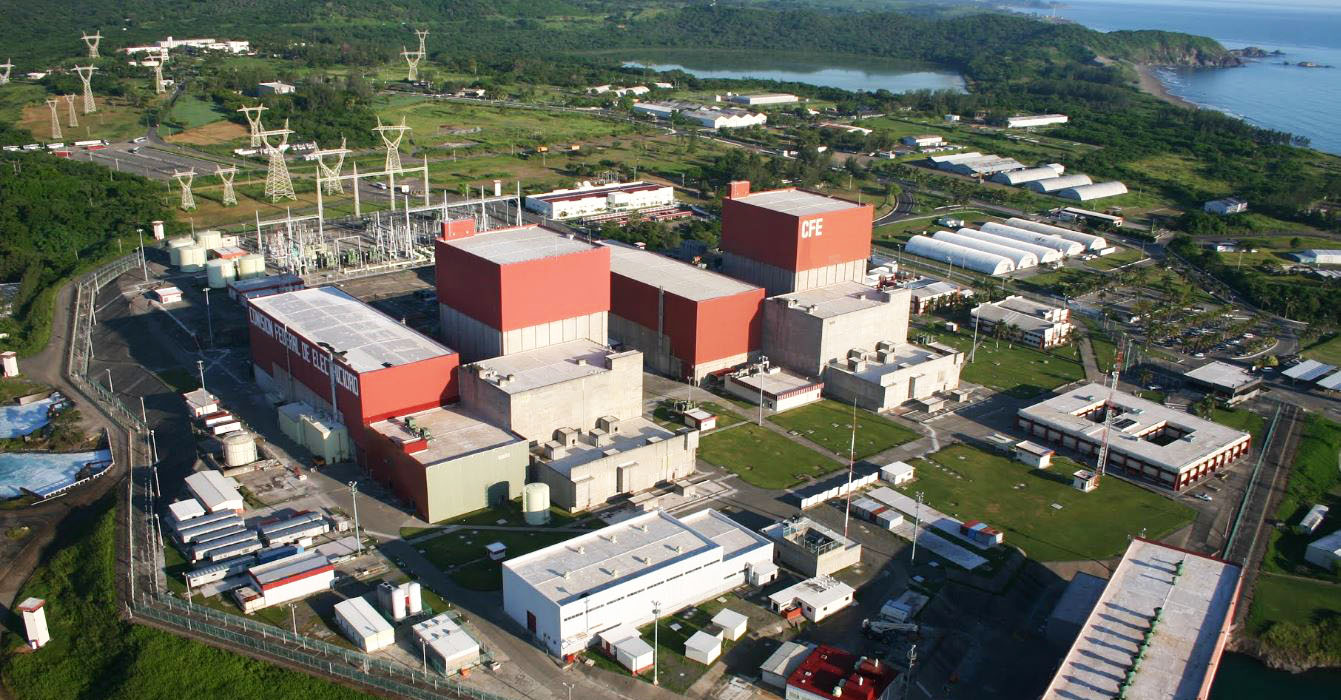
\includegraphics[width=\textwidth,trim=0pt 0pt 0pt 0pt,clip]{media/arie.jpg}
  \caption{An aerial view of the Laguna Verde power plant in Veracruz, Mexico. \cite{LVPIC}}
\end{figure}

The Laguna Verde Nuclear Power Plant is a boiling water reactor in Veracruz, Mexico. The reactor was designed, unfortunately, by General Electric, not Westinghouse. The power plant provides for roughly 4.8\% of Mexico's electricy production \cite{MEX} and is the only nuclear power plant in the nation. There are reactors at the site. The reactors follow the Rankine cycle. Water is pumped into the reactor vessel where it is heated by the reactor itself, this is our boiler, the increased pressure steam then turns turbines before it is cooled back down, condensed, and reintroduced to the cycle. A NRC report \cite{NRC} says the nuclear reactor's system "includes a direct cycle, forced circulation, boiling water reactor that produces steam for direct use in the steam turbine." This description highlights several components of our Rankine Cycle: forced circulation describes the work input done by the pump, boiling water reactor describes the boiler which increases pressure and temperature, and the turbine which produces the work output. Another key factor in this description is the reactor as being direct cycle. A direct cycle reactor passes water directly through the reactor, meaning the water is iraddiated. The water being irradiated means that the cycle must be closed; this gives us our final component, the condenser which converts the steam back into water. The principal aspect of the Rankine cycle is a phase change, and secondarily work output. The reactor's cycle fills these two aspects, in the reactor boiling the water and the turbine extracting work. 

\begin{figure}[H]
  \centering
  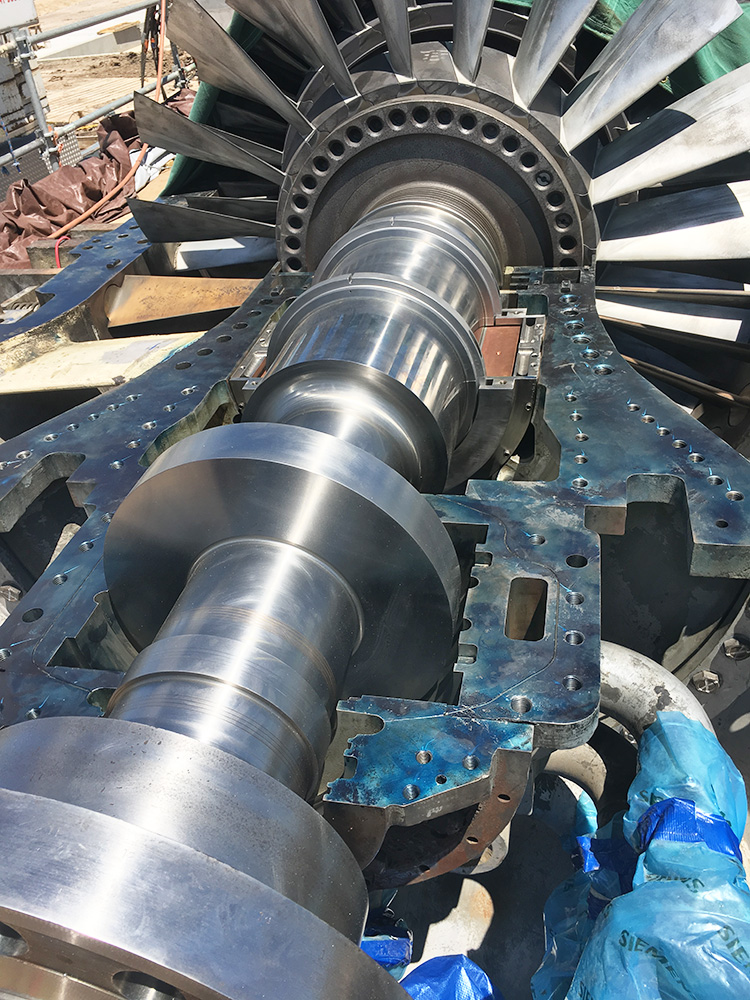
\includegraphics[width=0.5\textwidth,trim=0pt 0pt 0pt 0pt,clip]{media/turbine.jpg}
  \caption{A picture of the Westinghouse 501F gas turbine which is very similar to the kind used in the Sayreville Energy Center. \cite{TBPIC}}
\end{figure}


Another example of the Rankine cycle being used in power plants is the Sayreville Energy Center in Sayreville, New Jersey. The energy center was built by Westinghouse and Siemens Energy but is now operated by NextEra Energy Resources \cite{SA1}. The site uses a Combined Cycle Gas Turbine. The primary cycle of this type of power plant is the Brayton cycle, but the Rankine cycle is used for bottoming, to increase the efficiency of the plant. The first cycle burns the gas and this turns turbines which produce electricity. In the second cycle, the bottoming cycle, the exhaust is used to boil water which then is used to turn turbines and is recycled. This second cycle is a Rankine cycle. This usage is critical to increasing the efficiency of power plants and can increase the efficiency by around 50\% \cite{TVA}.


\section{Problem Setup}

The given variables for our power plant analysis are the following:

Boiler pressure, $P_3 = 8$ MPa, condenser pressure, $P_1 = 10$ kPa, turbine inlet temperature, $T_3 = 480\degC$.

We can begin filling out the rest of the state variables by realizing that $P_2 = P_3$, $P_1 = P_4$, these are shown in Figures 2 and 3. As stated in the introduction, the cycle is isentropic through the pump, Point 1 to Point 2, and through the turbine, Point 3 and Point 4. This shows that $s_1 = s_2$ and $s_3=s_4$. The boiler converts the saturated liquid into a saturated vapor, $x_3 = 1.0$, after the condenser the medium is a saturated liquid, $x_1 = 0.0$.

The rest of the state variables were calculated in EES, alternatively these values could be looked up in state tables. Table 2 displays the results.

\begin{table}[H]
\centering
\stateTable
\caption{Summary of state variables.}
\end{table}

\section{Energy Analysis}

\begin{table}[H]
\centering
\anaTable
\caption{Summary of energy analysis.}
\end{table}


The equations, taken from a SFU lecture \cite{EQU}, used to analyze the power plant Rankine cycle are listed below, the actual calculation was done in EES:

To calculate the turbine work output, $w_t$: 
\[w_t = h_3-h_4\]

To calculate the pump work input, $w_p$: 
\[w_p = h_2-h_1\]

To calculate the heat input to the boiler, $q_{\tn{in}}$: 
\[q_{\tn{in}} = h_3-h_2\]

To calculate the heat rejected in the condenser, $q_{\tn{out}}$:
\[q_{\tn{out}} = h_4-h_1\]

To calculate the net-work output from the cycle, $w_{\tn{net}}$: 
\[w_{\tn{net}} = q_{in}-q_{out}\]

To calculate the efficiency of the cycle, $\eta_{\tn{th}}$: 
\[\eta_{\tn{th}} = \frac{w_{\tn{net}}}{q_{\tn{in}}}\]

\subsection{Diagrams}

\begin{figure}[H]
  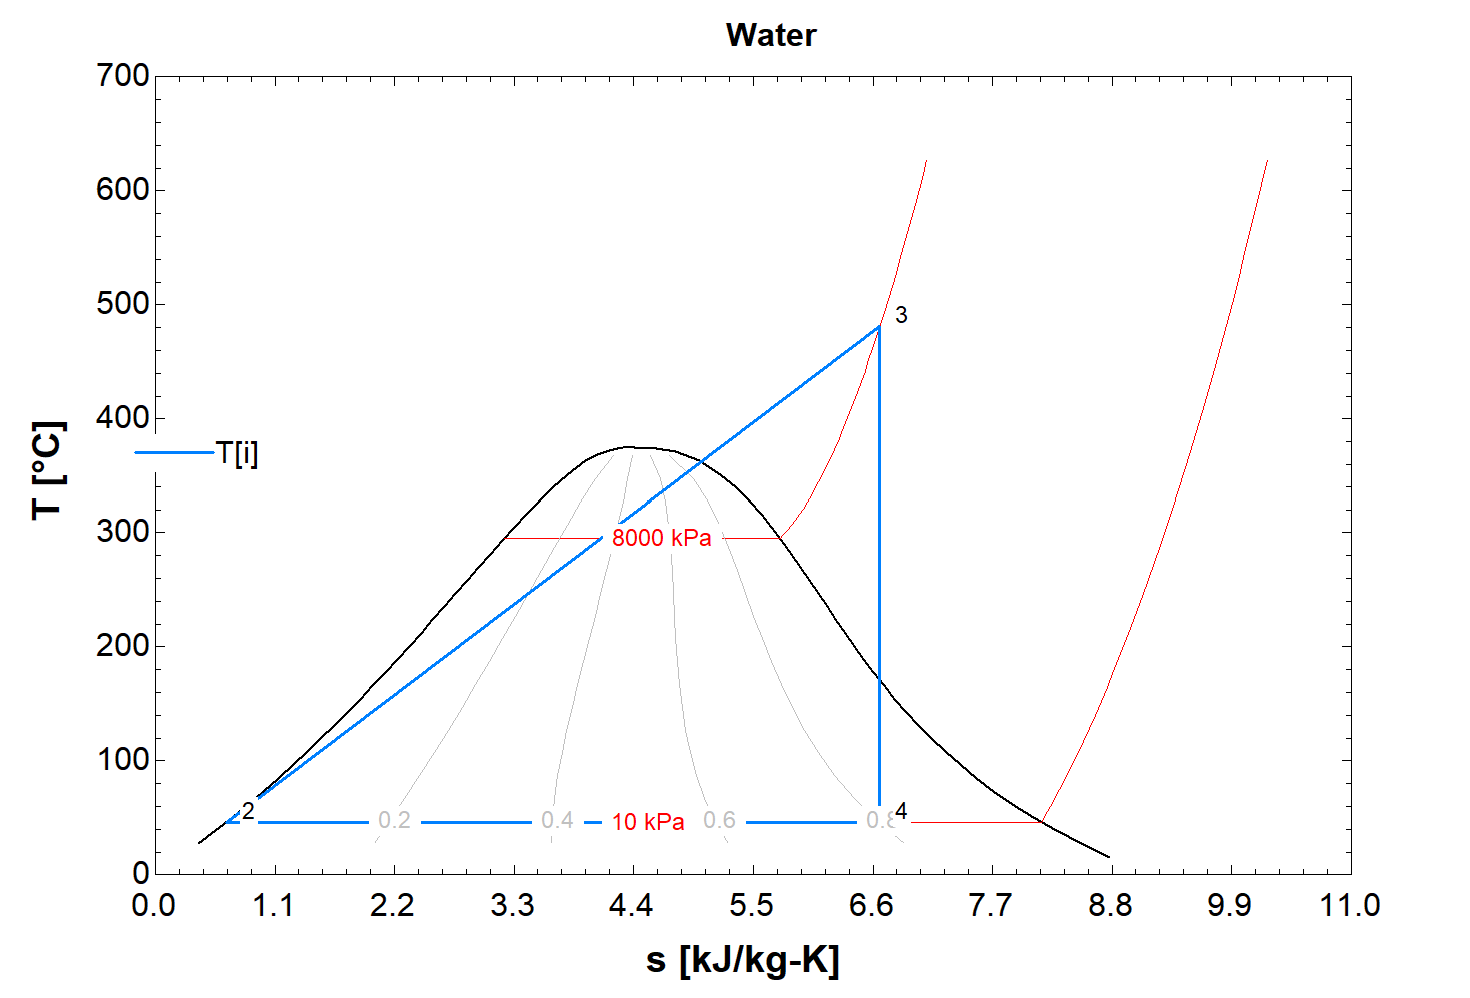
\includegraphics[width=\textwidth,trim=0pt 0pt 0pt 50pt,clip]{media/Ts.png}
  \caption{T-s diagram of the Rankine cycle using water. Point 1 is hidden by Point 2 as they are, relative to the scale, close together. The blue lines approximately show the cycle path. The red line at $P=8000$ kPa is a more accurate representation of the path, as Figure 3 shows us that pressure is constant from Point 2 to Point 3, and Figure 2 demonstrates that the shape of the red line is what we should expect. The black line is the saturation bell.}
\end{figure}


\begin{figure}[H]
  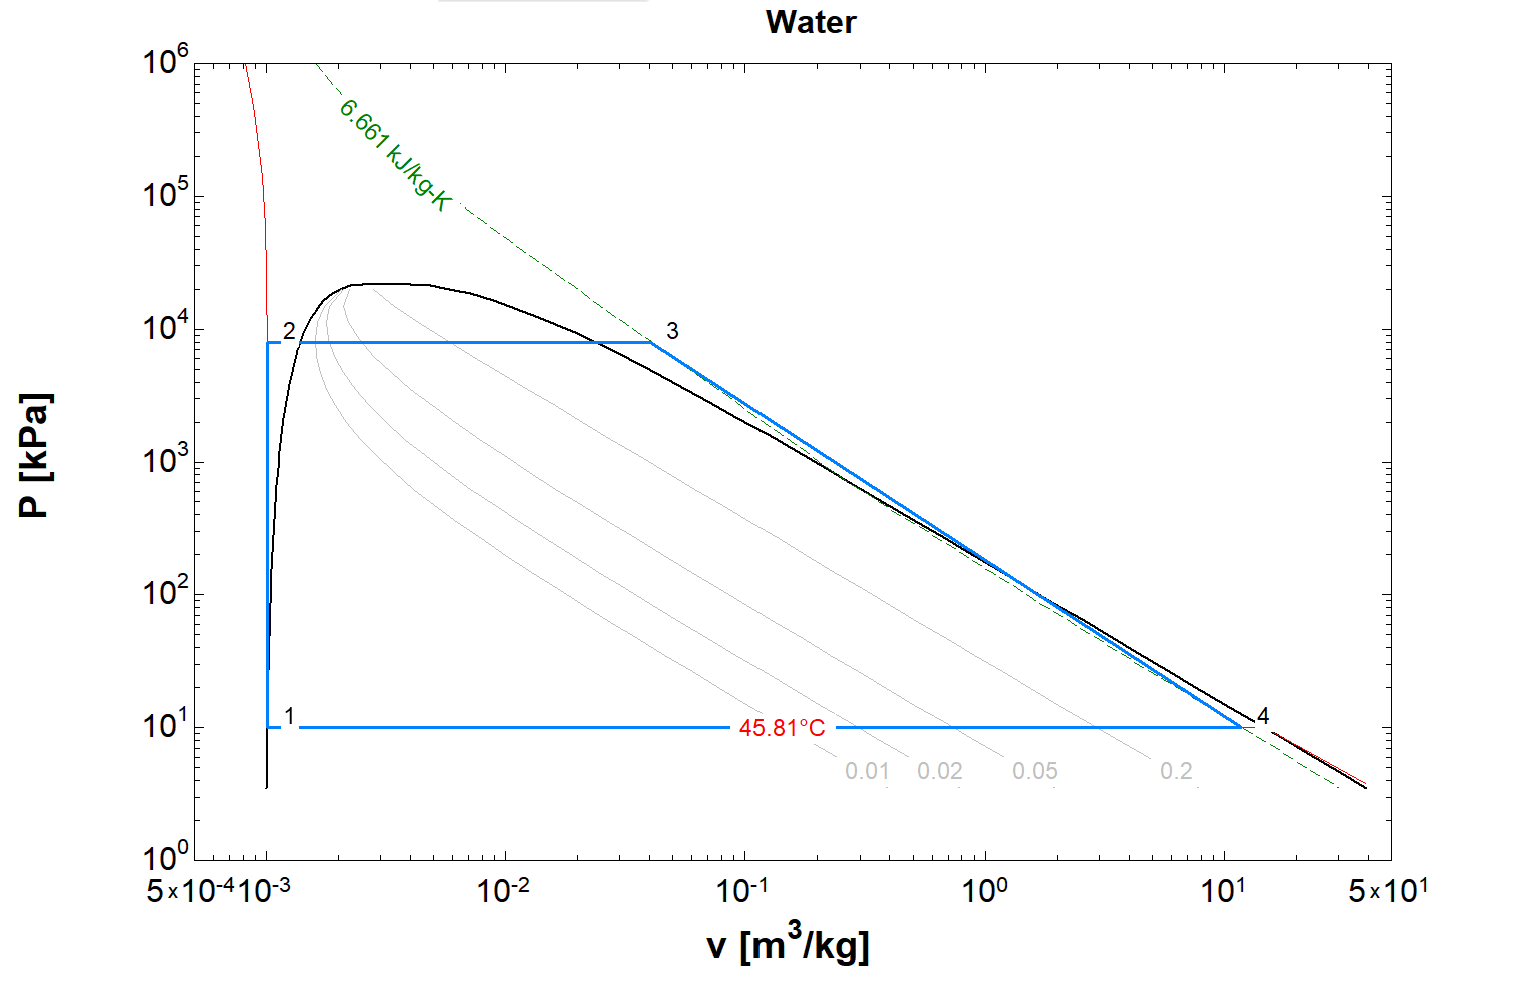
\includegraphics[width=\textwidth,trim=0pt 0pt 0pt 50pt,clip]{media/Pv.png}
  \caption{P-v diagram of the Rankine cycle using water. The blue lines approximately show the cycle path. The cycle from Point 3 to Point 4 is better shown by the entropy line, which is shown dotted in green, because entropy at these points is constant. The black line is the saturation bell.}
\end{figure}

Figure 5 demonstrates the principal factor of the Rankine cycle, the phase changes. In Figure 5 the cycle path starts at Point 1 with a quality of 0.0, a saturated liquid, it climbs outside, to the left of, the saturation bell at Point 2 where it becomes a compressed liquid, compressed by the pump. From Point 2 to Point 3 the path enters back under the saturation bell and comes outside above and to the right of saturation bell; the boiler converts the compressed liquid into a saturated vapor with quality 1.0. From Point 3 to Point 4 it enters back under the saturation bell, with a quality of 0.80.


\section{Parametric Study}

\begin{figure}[H]
  \centering
  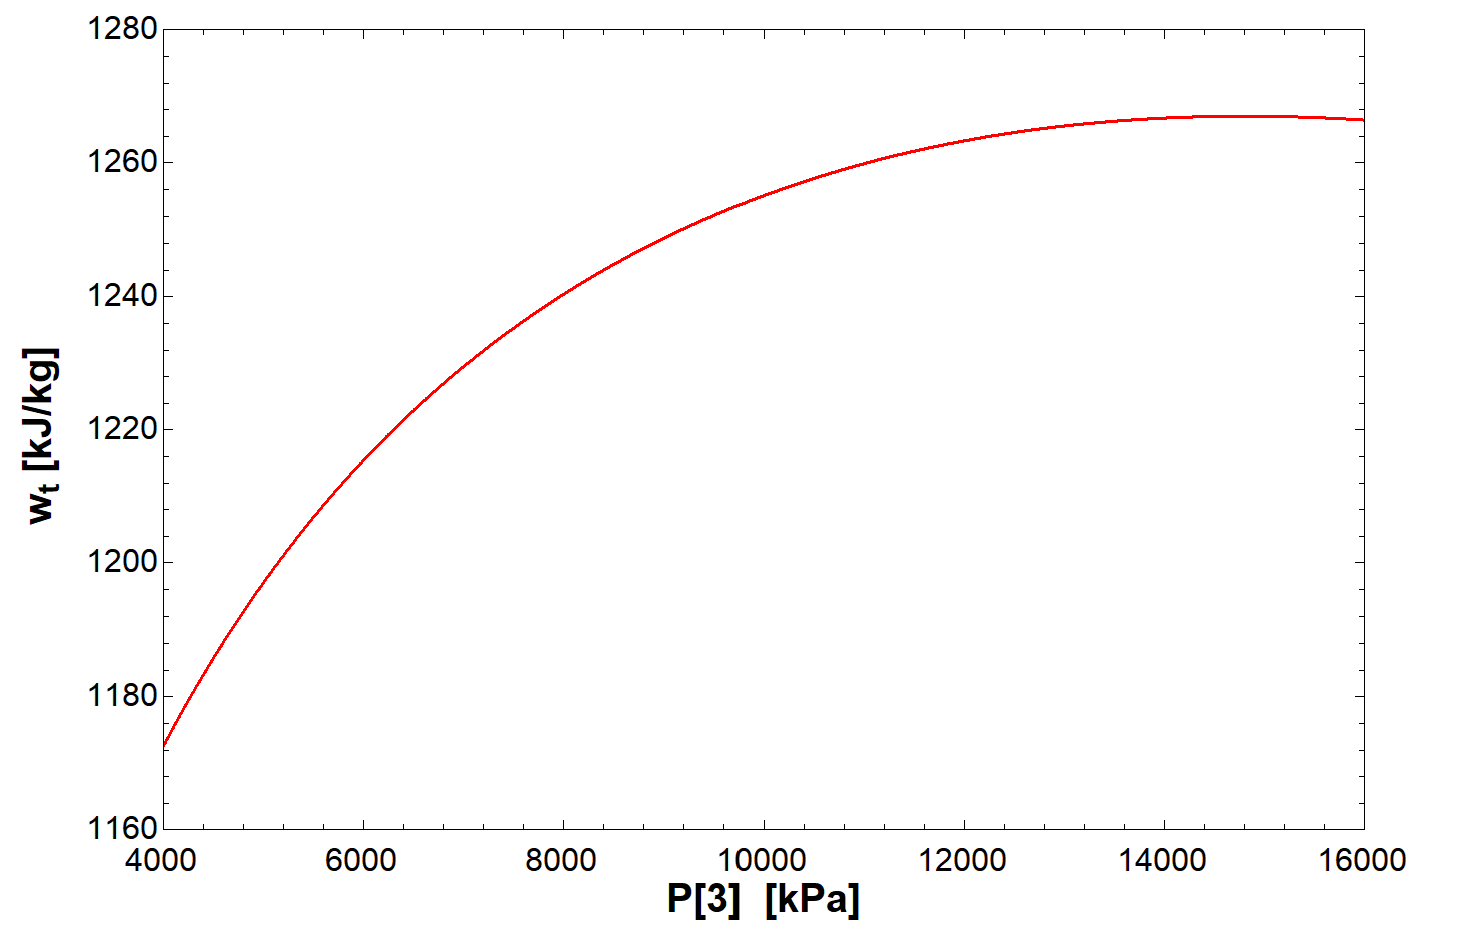
\includegraphics[width=\textwidth,trim=0pt 0pt 0pt 0pt,clip]{media/parametric.png}
  \caption{Parametric, work done by the turbine work output as affected by variable pressure exiting the boiler.}
\end{figure}

\begin{figure}[H]
  \centering
  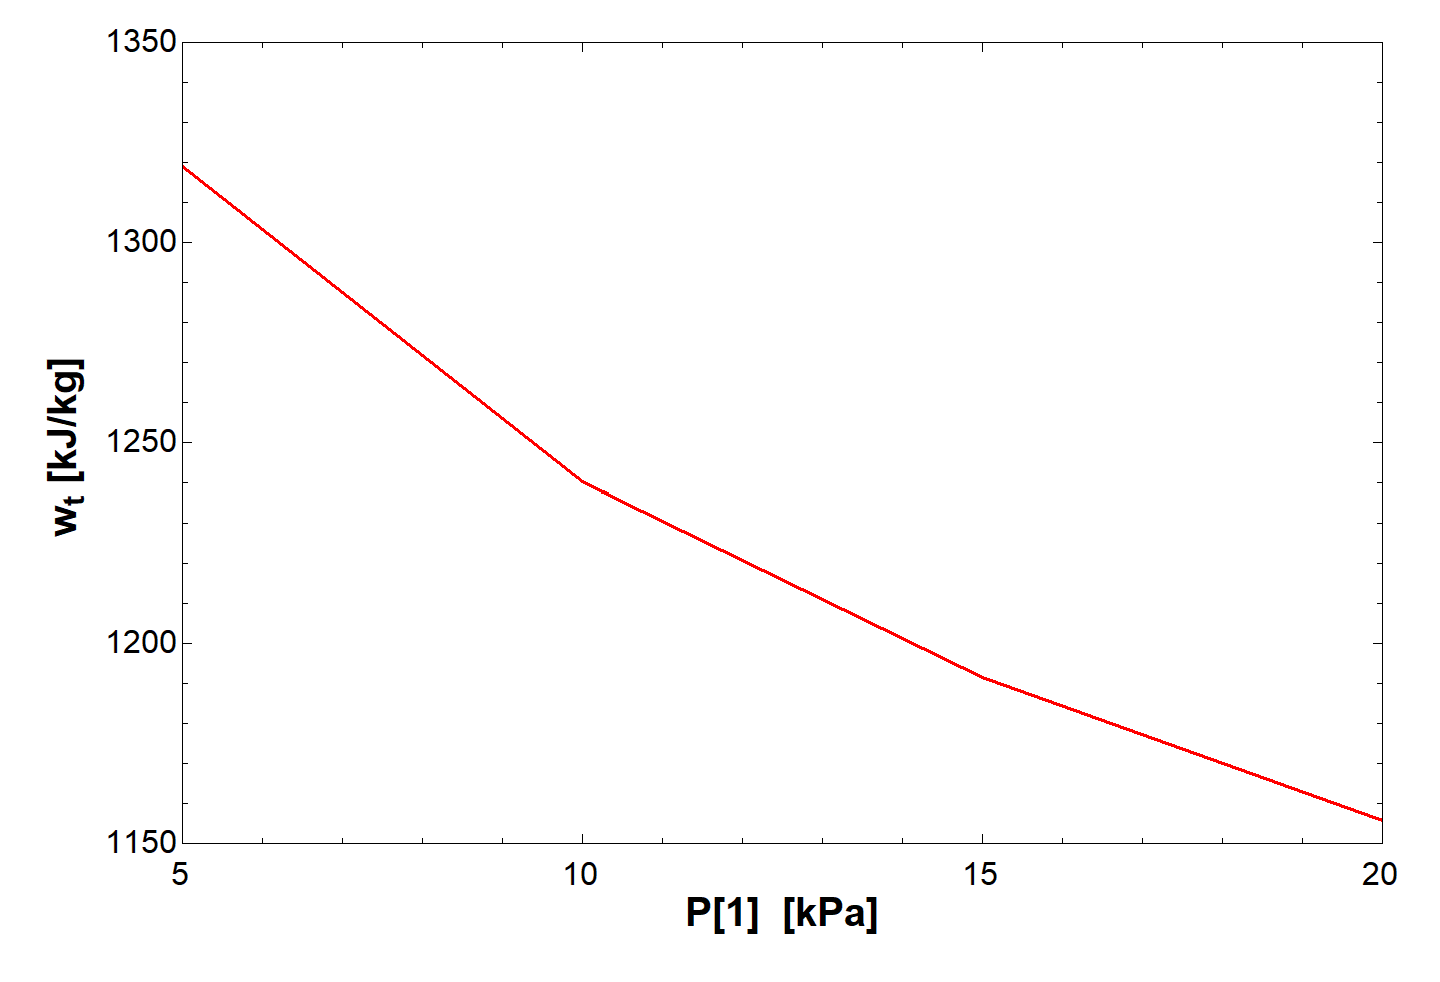
\includegraphics[width=\textwidth,trim=0pt 0pt 0pt 0pt,clip]{media/cond.png}
  \caption{Parametric, Condenser Pressure x axis work done by turbine y axis. parametric graph, 4 intervals of pressure displayed on x axis}
\end{figure}

\begin{figure}[H]
  \centering
  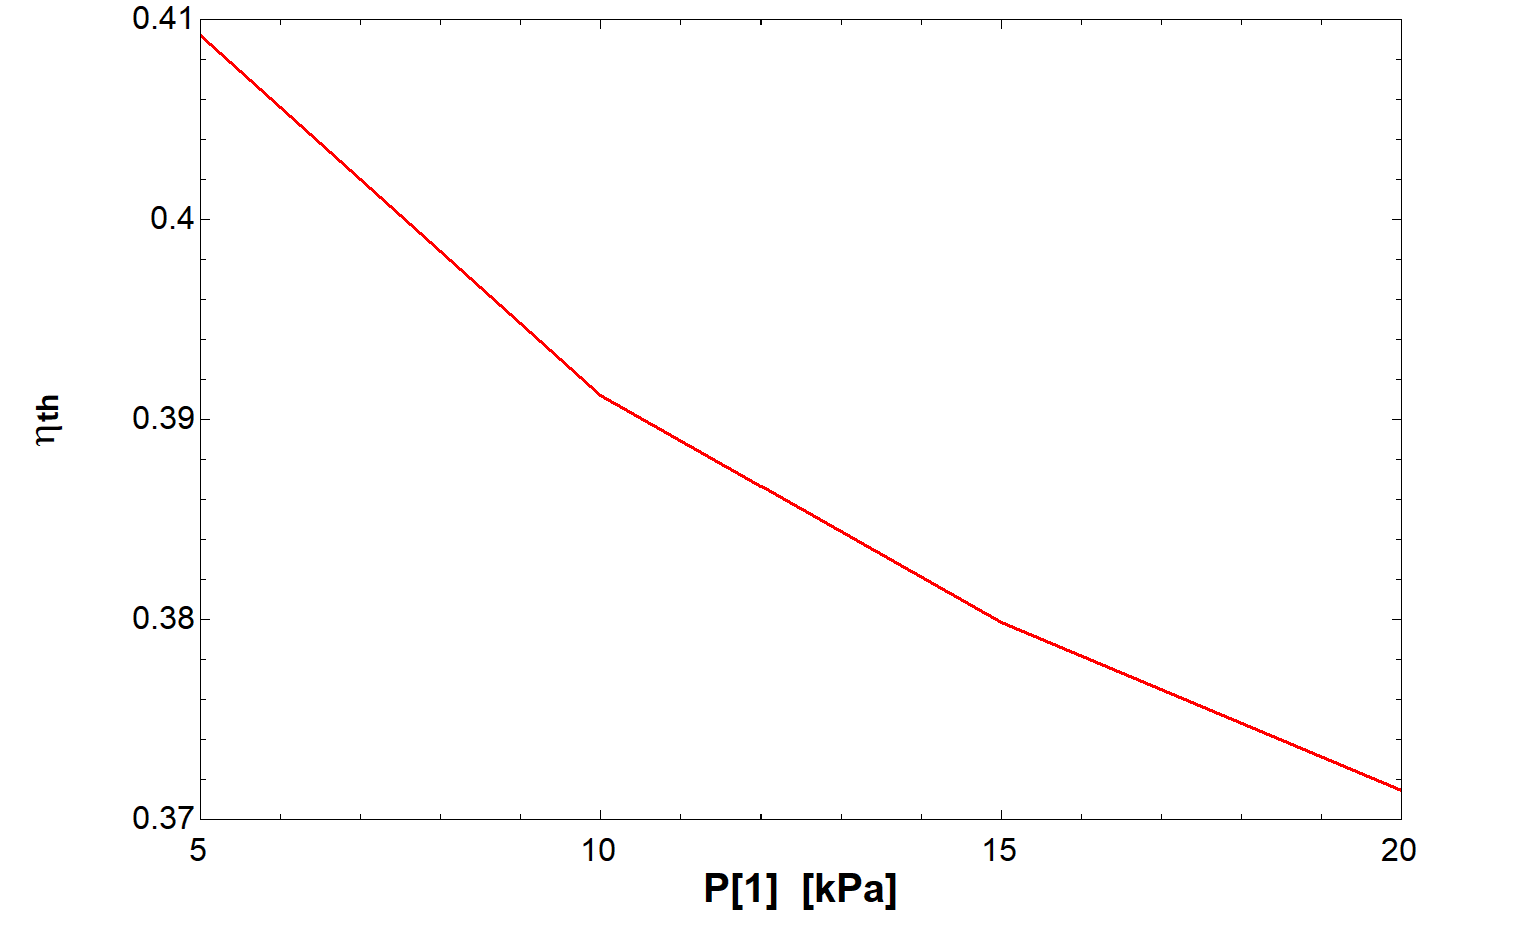
\includegraphics[width=\textwidth,trim=0pt 0pt 0pt 0pt,clip]{media/contherm.png}
  \caption{Parametric, efficiency (thermal) as affected by condenser pressure)}
\end{figure}

\begin{figure}[H]
  \centering
  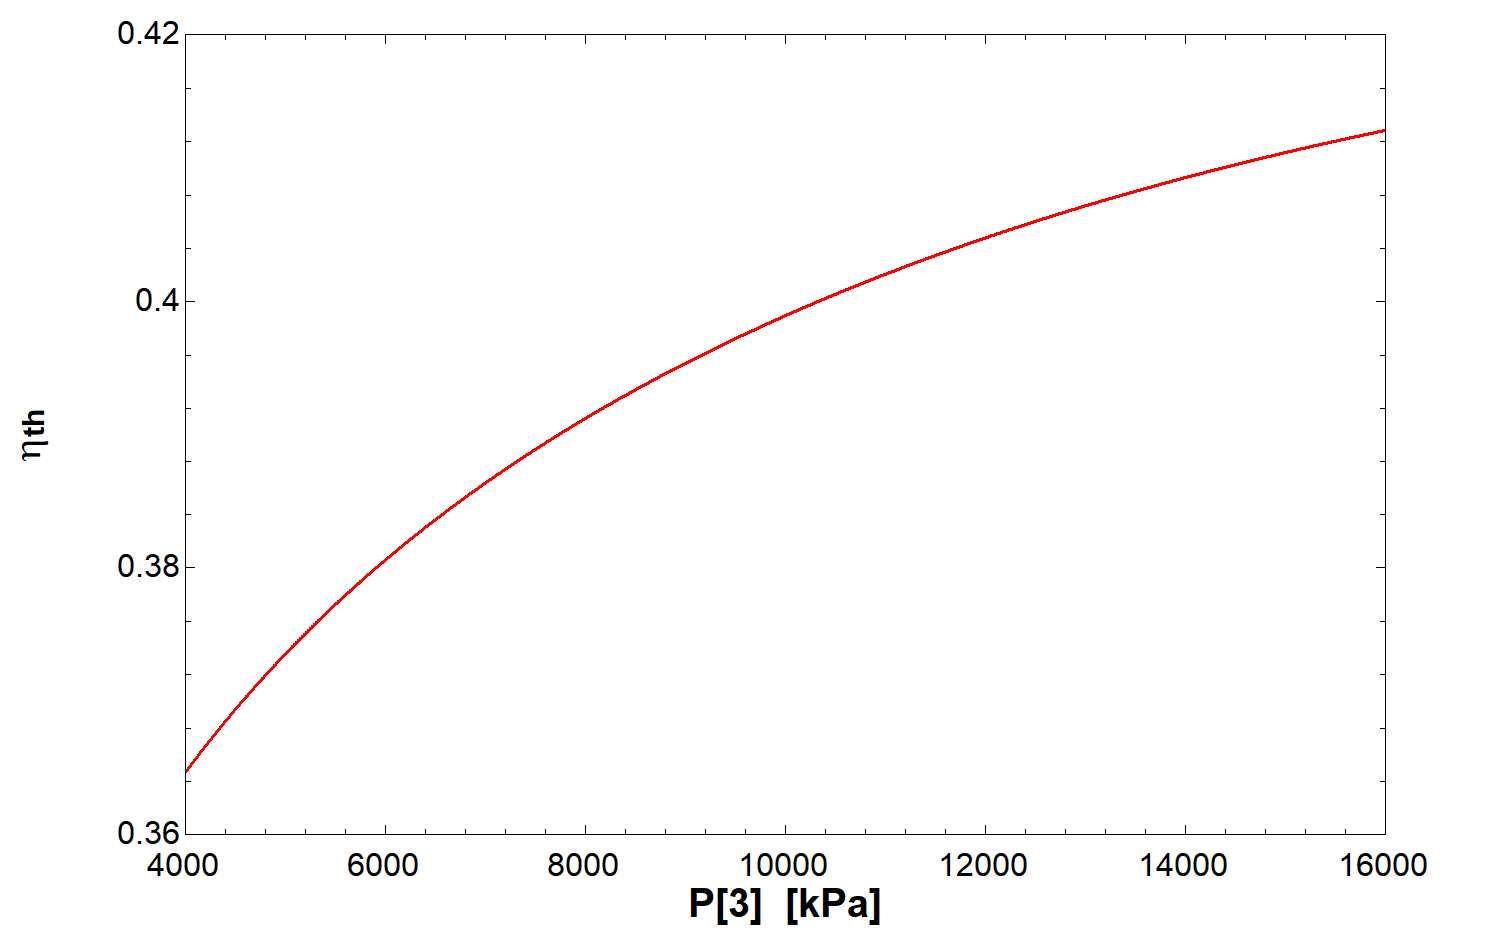
\includegraphics[width=\textwidth,trim=0pt 0pt 0pt 0pt,clip]{media/efftherm.png}
  \caption{Parametric, Thermal efficiency as affected by boiler pressure}
\end{figure}

\begin{figure}[H]
  \centering
  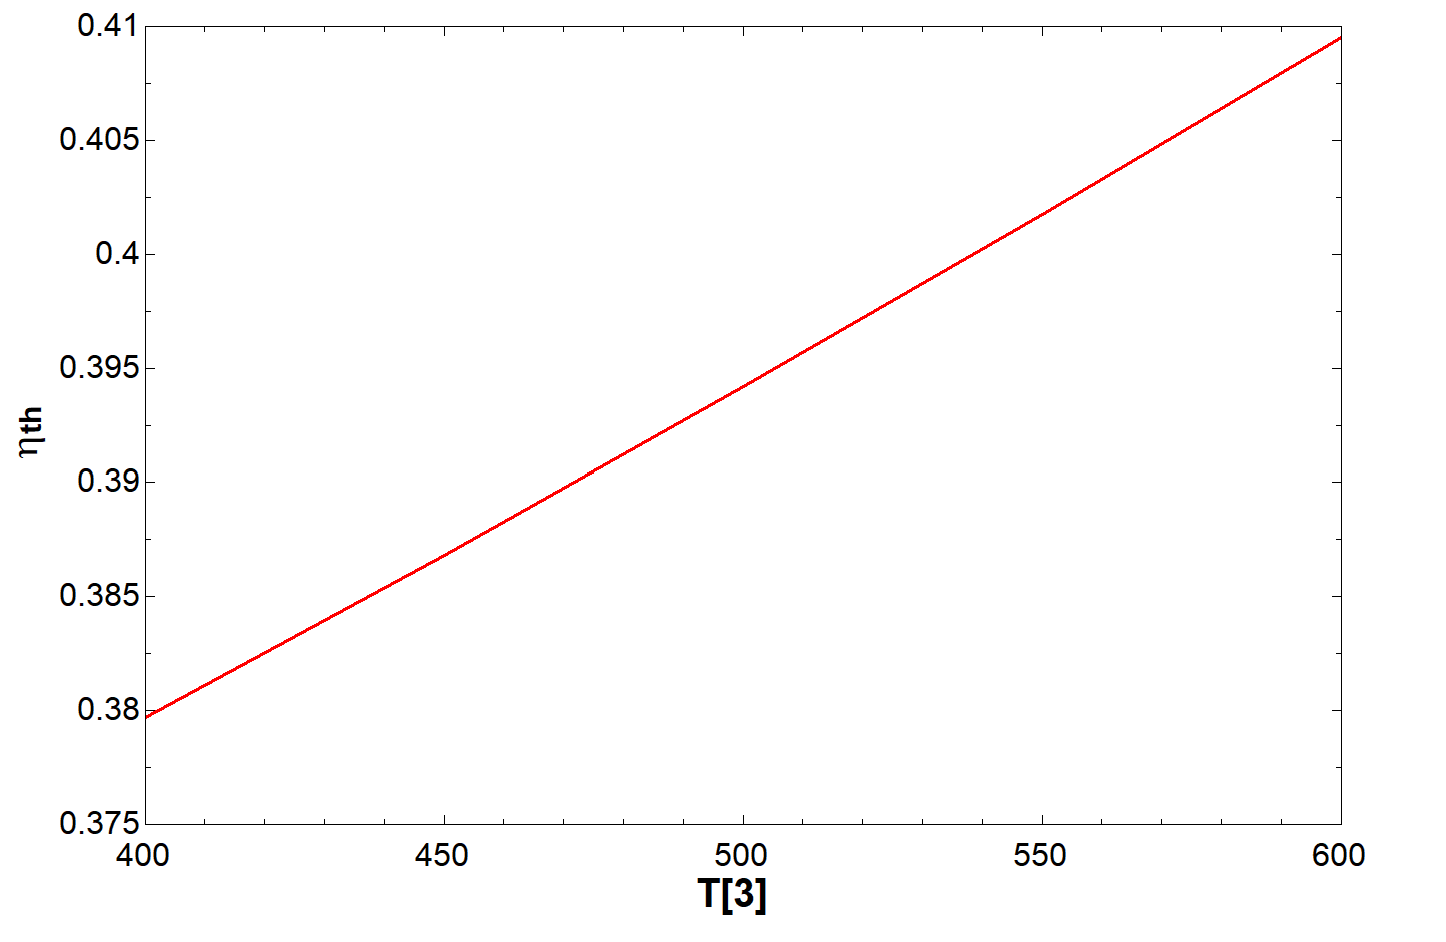
\includegraphics[width=\textwidth,trim=0pt 0pt 0pt 0pt,clip]{media/temtherm.png}
  \caption{Parametric, thermal efficiency as affected by temperature at boiler exit}
\end{figure}

\begin{figure}[H]
  \centering
  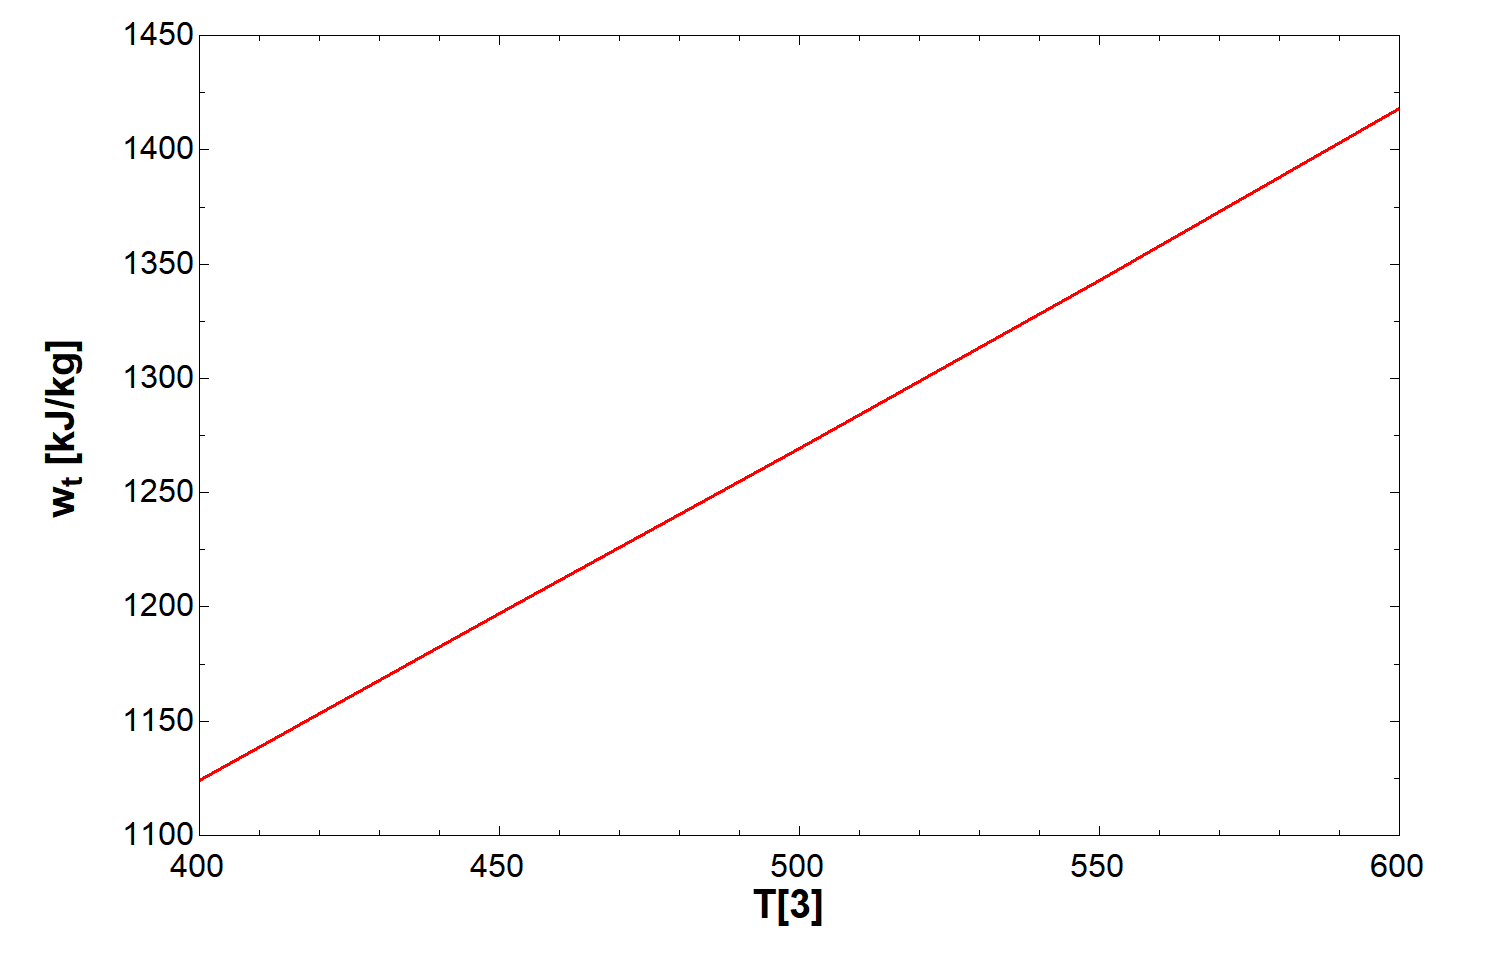
\includegraphics[width=\textwidth,trim=0pt 0pt 0pt 0pt,clip]{media/temwork.png}
  \caption{Parametric, work done by turbine (work out w/ units) as affected by boiler temperature (5 intervals of temp displayed on x-axis)}
\end{figure}



\section{Discussion}
\section{Conclusion}

\bibliographystyle{ieeetr} 
\bibliography{references} 

\end{document}
